\documentclass[10pt,a4paper]{article}
\usepackage[utf8]{inputenc}
\usepackage[czech]{babel}
\usepackage[T1]{fontenc}
\usepackage{graphicx}

\title{Cvičení číslo 3}
\author{Jakub Kadlčík}
\date{7. 10. 2013}

\begin{document}
	\maketitle
	\tableofcontents
	
	\section{Úvod}
	V kapitole číslo \ref{seznam-s-odrazkami} je ukázka seznamu s odrážkami. V kapitole číslo \ref{cislovany-seznam} je ukázka číslovaných seznamů. Poslední kapitola se zabývá seznamy pojmů. Najdeme ji na \pageref{seznam-pojmu}. straně. Závěrečná \ref{obrazky}. kapitola obsahuje dva obrázky. Rovnou si procvičíme i poznámky pod čarou a křížové odkazy \footnote{Čísla kapitol a stránek se v tomto textu doplňují automaticky}.
	
	\section{Seznam s odrážkami}
	\label{seznam-s-odrazkami}
	\begin{itemize}
		\item Pro seznamy s odrážkami slouží prostředí itemize
		\item Každá položka v seznamu začíná příkazem \textbackslash{}item \footnote{Odrážka může být libovolný znak}
		\item[$\circ$] circ
		\item[$\cdot$] cdot	
		\item[$\star$] star
		\item[$\ast$] ast
		\item[$\rightarrow$] rightarrow
		\item[$\diamondsuit$] diamondsuit
		\item[*] Hvězdička
	\end{itemize}
	
	\section{Číslované seznamy}
	\label{cislovany-seznam}
		\subsection{Standardní styl číslování}
			\begin{enumerate}
				\item První
				\item Druhý
				\item Třetí
					\begin{enumerate}
						\item První
						\item Druhý
						\item Třetí
					\end{enumerate}
				\item Čtvrtý	
			\end{enumerate}

		\subsection{Používáme vlastní styl}
			\begin{enumerate}
				\renewcommand{\labelenumi}{\arabic{enumi}.}
				\renewcommand{\labelenumii}{\arabic{enumi}.\arabic{enumii}.}
				\renewcommand{\labelenumiii}{\arabic{enumi}.\arabic{enumii}.\arabic{enumiii}.}
				\item První
				\item Druhý
				\item Třetí
					\begin{enumerate}
						\item První
						\item Druhý
						\item Třetí
							\begin{enumerate}
								\item První
								\item Druhý
								\item Třetí
							\end{enumerate}
					\end{enumerate}
				\item Čtvrtý	
			\end{enumerate}
			
		\subsection{Další možný styl číslování}
		Psát nebudu, protože už se mi nechce
		
	\section{Seznam pojmů}
	\label{seznam-pojmu}
	\begin{description}
		\item[itemize] -- prostředí pro seznamy s odrážkami	
		\item[enumerate] -- prostředí pro číslované seznamy
		\item[description] -- prostředí pro seznam pojmů
	\end{description}
	
	\section{Obrázky}
	\label{obrazky}
		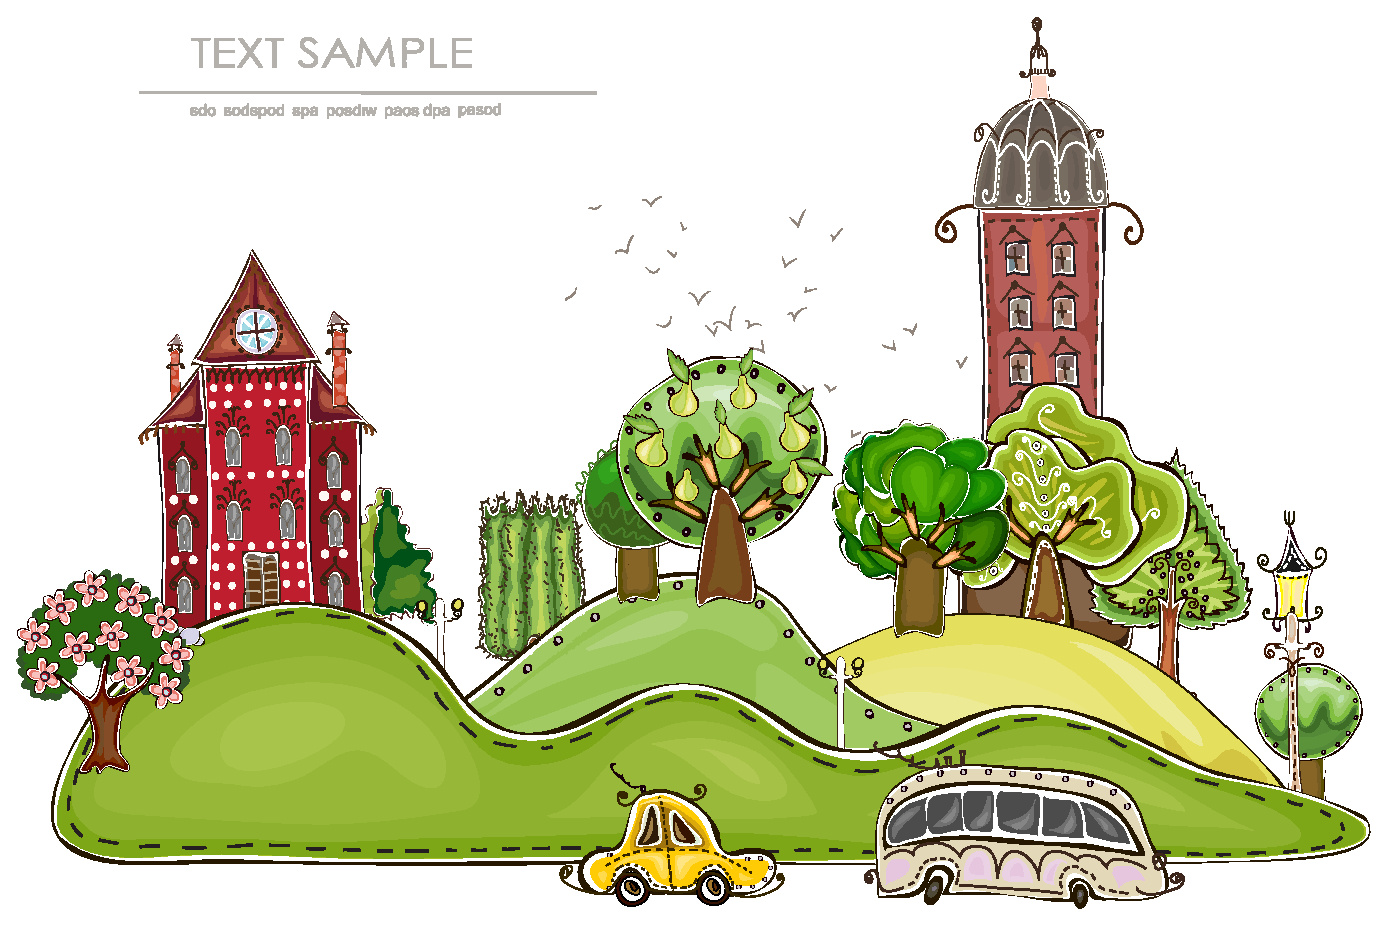
\includegraphics[scale=0.60]{Obrazek1.eps}
		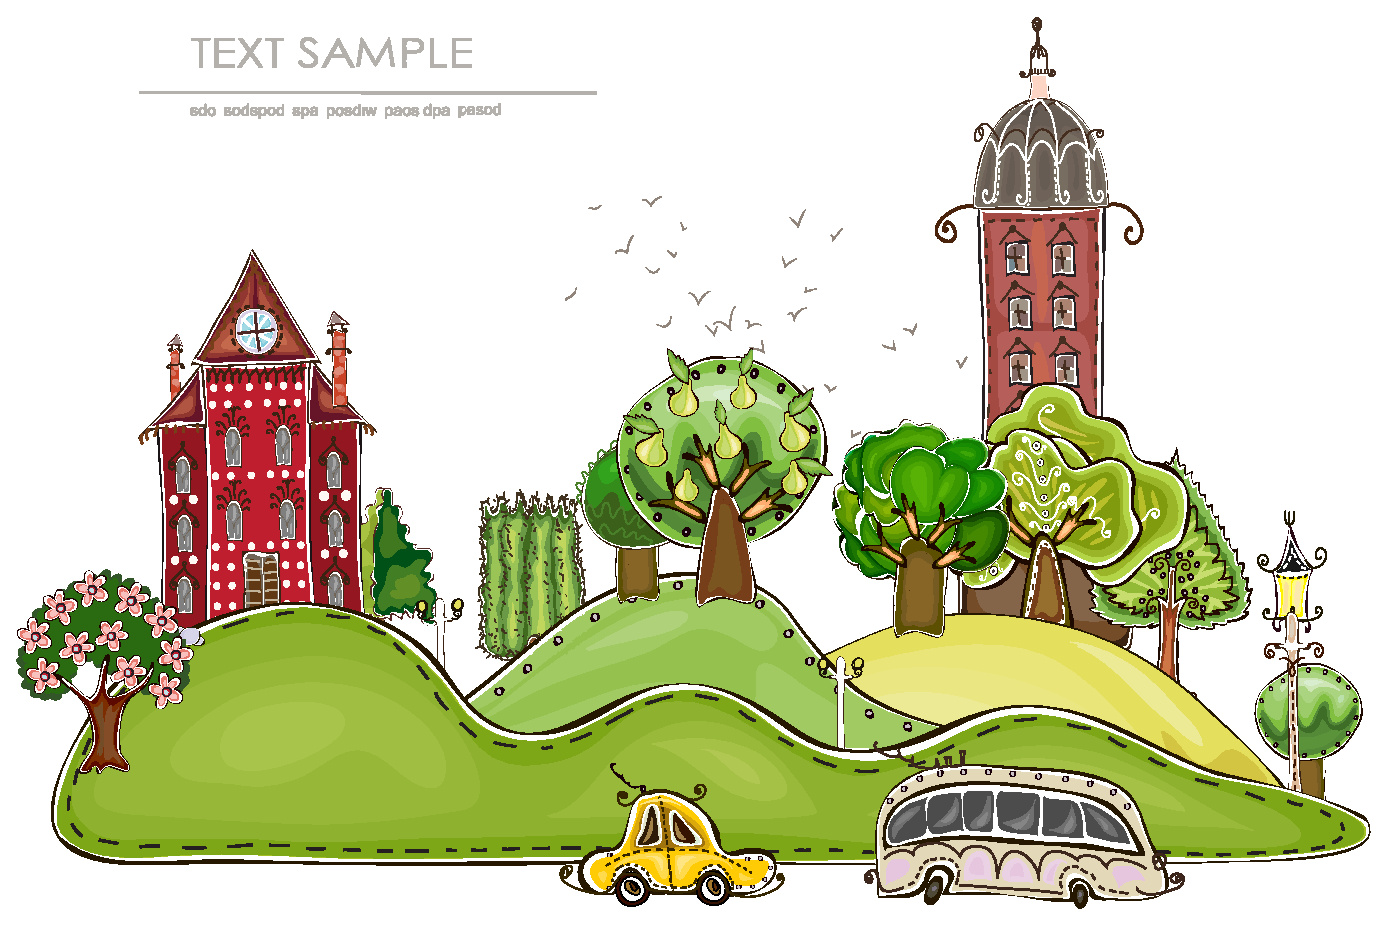
\includegraphics[width=5cm, angle=-40]{Obrazek1.eps}
\end{document}